\chapter{Background}\label{sec:background}
\begin{quote}
    In this chapter, we recapitulate the foundations which are used to build on in this work.
    In Section \ref{sec:representation_learning}, we discuss common approaches to representation learning.
    We first discuss the intuition behind an upcoming learning paradigm, self-supervised learning, in Section \ref{sec:self_supervised_learning} and highlight  the literature and challenges on self-supervision on audio data in Section \ref{sec:self_supervision_audio}. After providing a general intuition behind this learning method, we dive into self-supervised contrastive learning in section \ref{sec:contrastive_learning}, in which a gentle theoretical foundation is provided and two self-supervised contrastive learning frameworks are discussed. In Section \ref{sec:conv_audio}, we discuss convolutional neural networks for raw audio signals.
    Finally, we discuss the task of music auto tagging and their evaluation metrics in Section \ref{sec:task_description}.
\end{quote}


\section{Representation Learning}\label{sec:representation_learning}
% The performance of machine learning models is heavily dependent on the choice of features and representations.
% Features are often engineered using human intuition and domain knowledge of the composition of the input data, i.e., feature engineering.
% While feature engineering can greatly help to improve model performance, it is time-consuming and highlights the inability of traditional learning algorithms to identify and disentangle explanatory factors hidden in high-dimensional signals.


The goal of representation learning is to identify features that make  prediction tasks easier and more robust to the complex variations of natural data \cite{bengio2013representation}.
Supervised techniques for representation learning have now been successfully applied to a variety of tasks in the audio domain, e.g. rhythm detection, musical key recognition, chord recognition, music auto tagging, speaker identity recognition and phoneme recognition  \cite{korzeniowski_fully_2016, chen_harmony_2019, korzeniowski_end--end_2017, bock_joint_2016, pons_end--end_2017, van_den_oord_deep_2013}. We first give a brief overview of three main strategies of learning:

% In the unsupervised domain, generative modeling and likelihood-based models use reconstruction of the observations as the objective for learning useful representations of the data.

\noindent\rule{\textwidth}{0.5pt}

\begin{itemize}
    \item \textbf{Supervised learning} uses (often) human-annotated labels as a guidance to learning an objective. This learning paradigm is (often) limited to the amount of manually annotated data that is available for training.
    \item \textbf{Unsupervised learning} is the set of algorithms that do not exploit pre-annotated labels.
    \item \textbf{Reinforcement learning} uses agents that maximise their reward in an environment by performing sequences of actions to learn an objective. Learning is unguided in the sense that suboptimal actions are not explicitly corrected by a supervisory signal.
\end{itemize}

\noindent\rule{\textwidth}{0.5pt}

\begin{marginfigure}[{0cm}]
    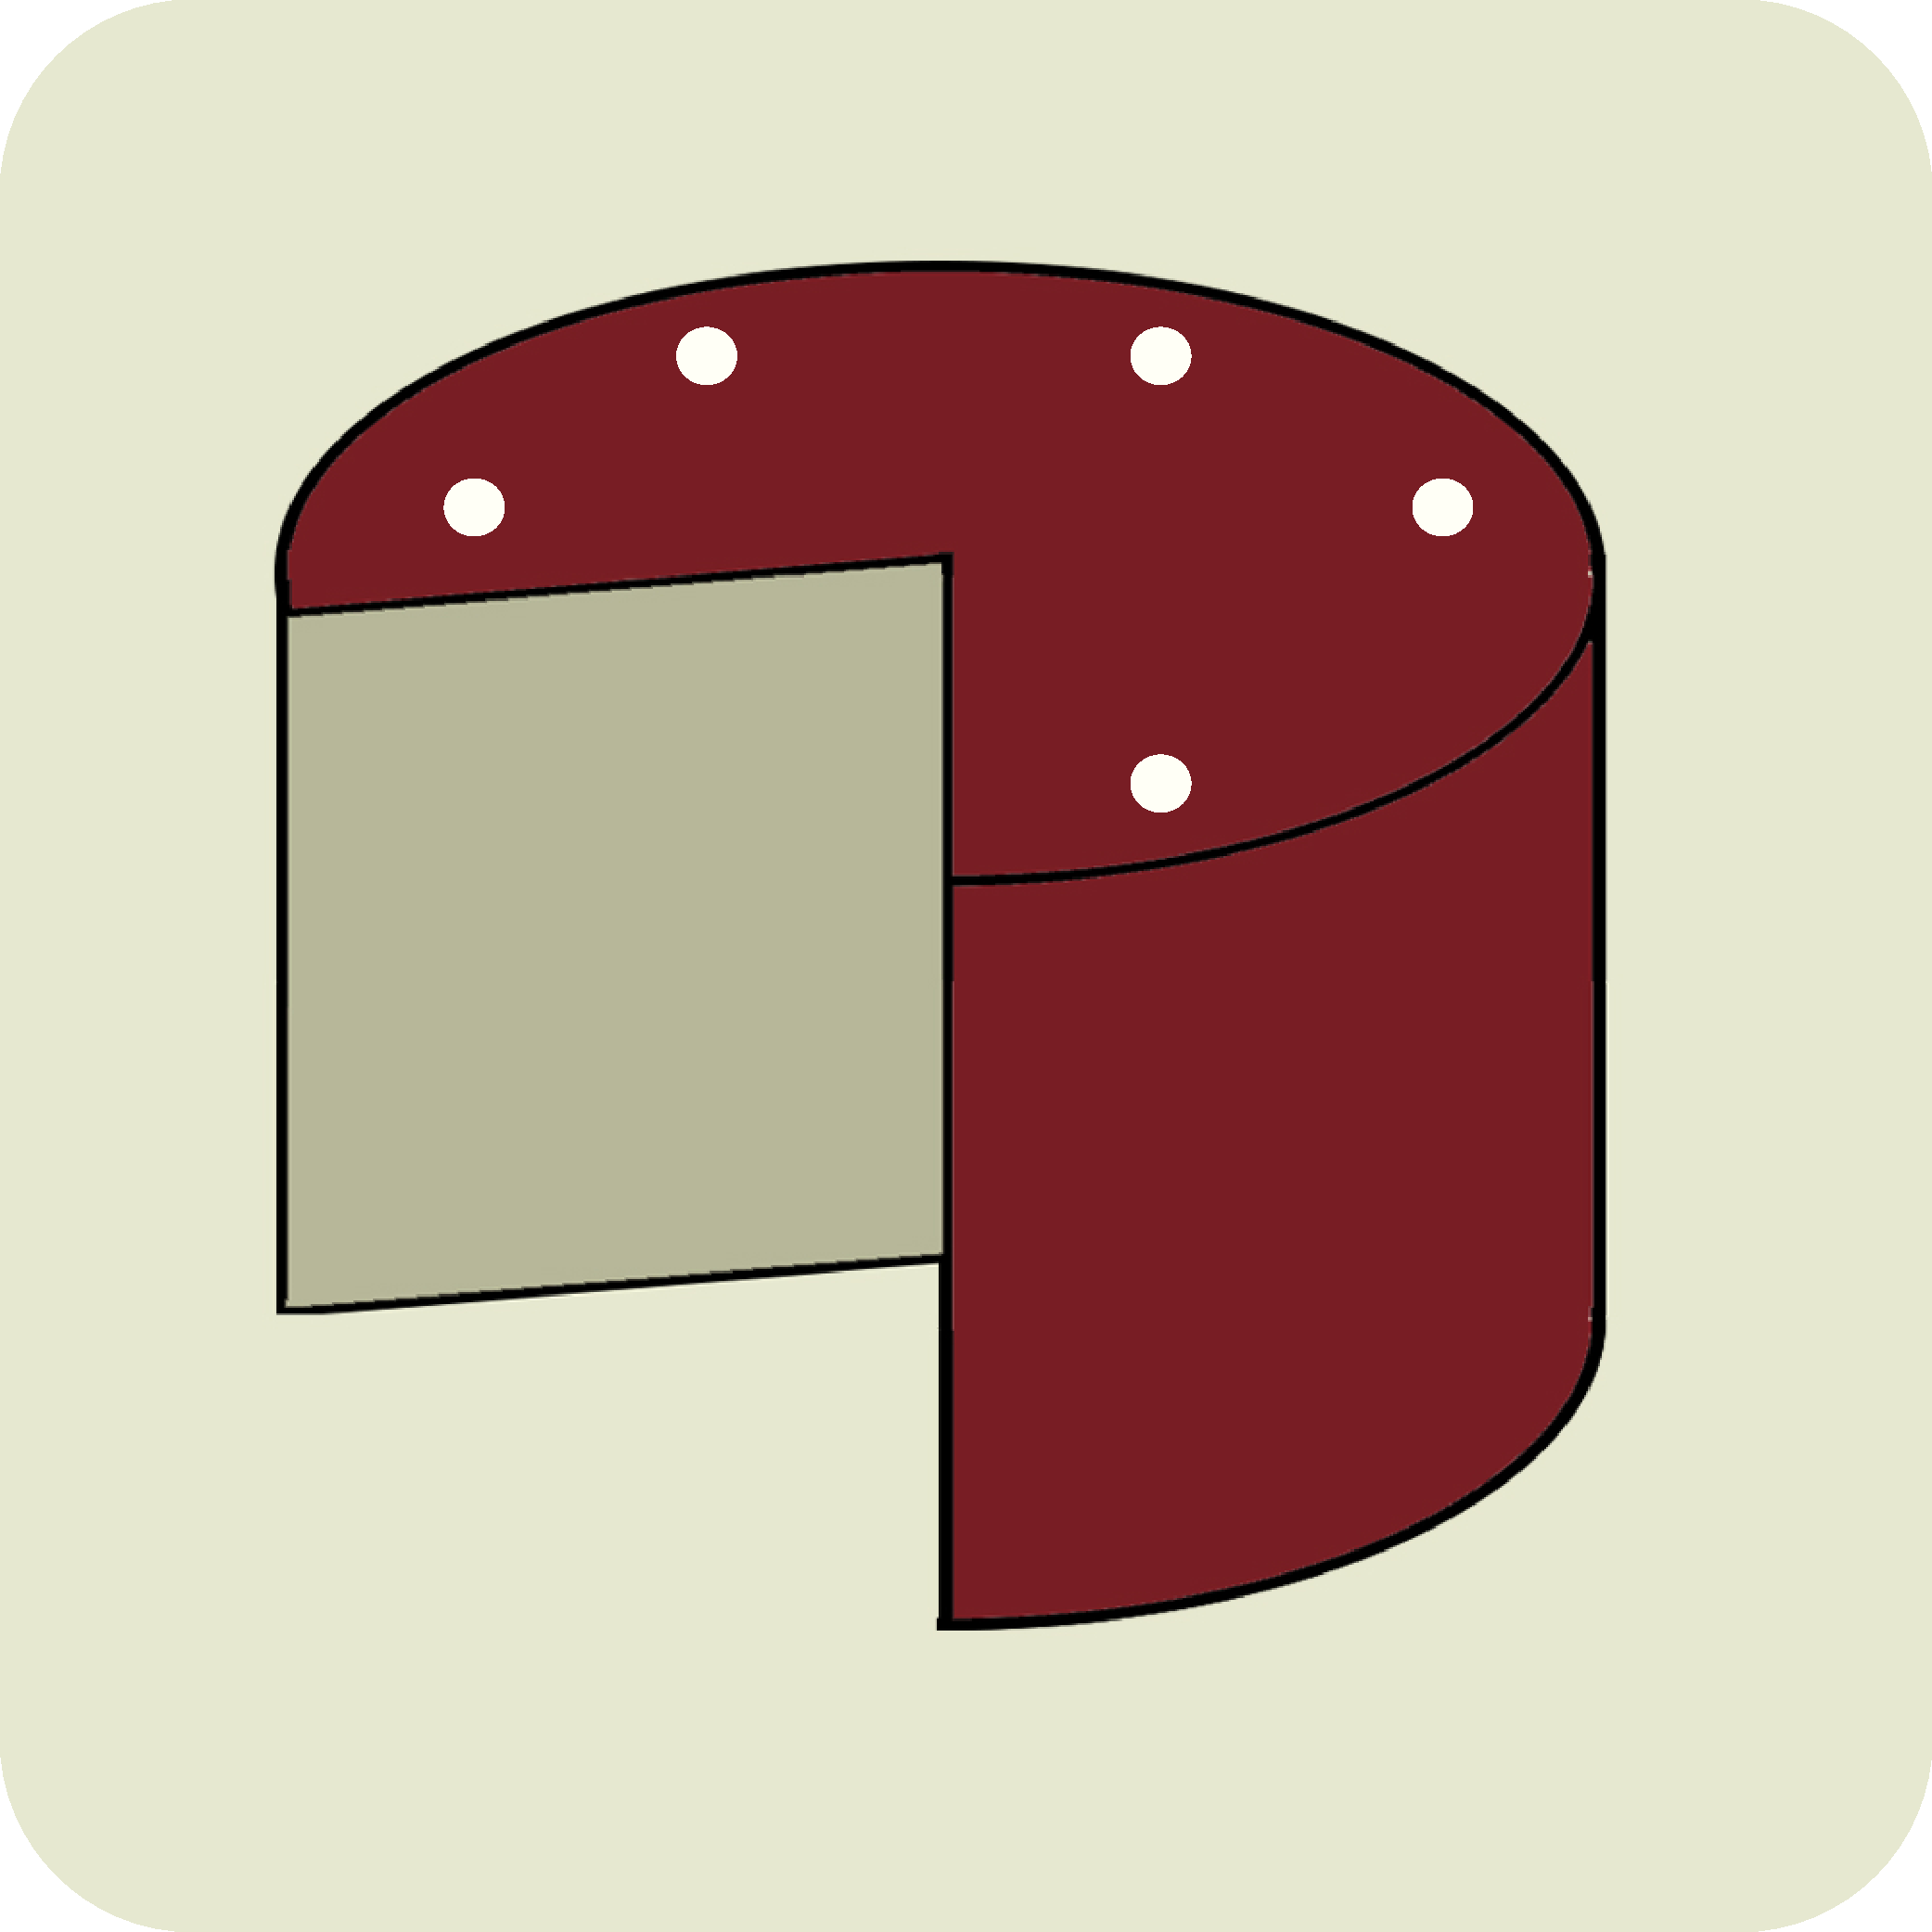
\includegraphics[width=\textwidth]{figs/cake_analogy.pdf}
    \caption{Yann LeCun, a strong advocate of unsupervised learning, famously introduced the `cake analogy' at NIPS 2016: \textit{``If intelligence is a cake, the bulk of the cake is unsupervised learning, the icing on the cake is supervised learning, and the cherry on the cake is reinforcement learning.''}}
    \label{fig:cake_analogy}
\end{marginfigure}



We also highlight the difference between between two learning methods that fall under the unsupervised learning paradigm to avoid confusion:
\begin{itemize}
    \item Semi-supervised learning is a learning paradigm that manifests itself between unsupervised and supervised learning. It uses few supervisory signals to guide training using many unlabeled data points. 
    \item Self-supervised learning is a form of unsupervised learning that formulates the learning objective in such a way, that it retrieves a supervisory signal from (transformations of) the data itself.
\end{itemize}


The distinguishment between learning methods in the unsupervised learning domain can be daunting at first, e.g., generative modeling and likelihood-based models are considered unsupervised learning methods that typically find useful representations of the data by attempting to reconstruct the observations on the basis of their learned representations \cite{goodfellow2014generative, unsupervised_gan}.
Broadly speaking, these approaches can also be considered as self-supervised representation learning: the objective is formulated in such a way that it gets supervision from the data itself.
The difference between generative approaches and self-supervised learning we like to distinguish, is that self-supervised learning aims to identify the explanatory factors of the data using an objective that is formulated with respect to the representations directly, and its goal is not to generate a faithful reproduction of the data but rather to learn useful features for (multiple) downstream tasks.

In this thesis, our focus will be on the \textit{self-supervised} learning paradigm. We will first give an overview of its usage in different domains, as to sketch a clear image of its workings and the unique challenges in each domain, while work on self-supervised learning in audio is relatively limited.

\section{Self-supervised Learning}\label{sec:self_supervised_learning}
This idea of self-supervised learning has seen widespread adoption in language modeling.
Its most common task is to predict the next word, given a past sequence of words, but more auxiliary (pretext) tasks can be added to improve the language model.
For example, BERT \cite{Devlin2019BERTPO} adds two auxiliary tasks that both rely on self-generated labels to improve the bi-directional prediction of word tokens and sentence-level understanding: 1) a cloze test \cite{doi:10.1177/107769905303000401}, in which part of the tokens in each sequence is randomly masked and the model is asked to predict the missing tokens, and 2) optimising a binary classifier on predicting whether one sequence follows another sequence.
The first pretext task encourages the model to better capture the syntactic and semantic meaning of the context around a word, and the second task improves the understanding of relationships between sentences.
Building these tasks requires no manual labeling, and can therefore be scaled up to arbitrary size while there is plenty of free text available to use as training data.\\

\subsection{Formulation of pretext tasks}
In the image domain, self-supervised learning manifests itself in a similar way: one or multiple pretext tasks are formulated on a set of unlabelled images and, subsequently, the pre-trained encoder or its intermediate layers are used to fine-tune on a downstream task like image classification.
We first resort to the image domain that has enjoyed more attention than the field of audio research to give a more clear intuition of the types of pretext tasks that were devised to learn useful representations for downstream tasks.
We give a short description of five different approaches.

Exemplar-CNN \cite{dosovitskiy_discriminative_2014} creates a surrogate dataset by randomly applying a sequence of transformations to `exemplary' image patches that contain large gradients, e.g., image patches that contain edges, strong textures, i.e., objects or parts of objects of interest.
Its pretext task is to classify the corresponding class of each transformed image.

An even more simple pretext task is formulated in RotNet \cite{gidaris2018unsupervised}, that proposes to use a random 2d rotation transformation as a supervisory signal to learn semantic features of an image.
The image is randomly rotated and given a class label: no rotation, $90^\circ$, $180^\circ$ or $270^\circ$, making the pretext task a 4-class classification problem.
Arguably, this forces the model to learn relationships in the semantic space of objects, i.e., to recognize the same image under different rotations, it has to learn more high-level, structural parts of the image, e.g., the relative position of a nose with respect to the eyes.
RotNet drastically reduced the gap between unsupervised and supervised feature learning in the image domain using a simple pretext task.

Another common transformation is that of colorization \cite{zhang_colorful_2016}, in which they extracted the lighting channel \textit{L} from a colored image and subsequently asked the model to predict the corresponding $a$ and $b$ color channels in CIE \textit{Lab} colorspace.

A pretext task can also be formulated as a relationship between two random patches of a single image. In \cite{doersch2015unsupervised}, they exploit the spatial context of an image as a supervisory signal.
Again given a large set of unlabeled images, random pairs of patches are extracted from each image and the network is asked to predict the position of the second patch relative to the first patch\footnote{In contrast to Exemplar-CNN, sampling is done without regard to the content of the image.}.
A $3\times 3$ grid is constructed and, given the first patch is located in the center, the model is asked to predict the location of a patch located in any of the remaining 8 positions, turning the pretext task into an 8-class classification problem.\footnote{
Interestingly, this approach quickly found a trivial solution to the problem of identifying the relative position between a pair of images: chromatic aberration.
This phenomenon arises when a lens fails to focus light at different wavelengths \cite{brewster_treatise_1835}.
Convolutional neural networks are able to localise such patches relative to the lens, which makes the objective of identifying the relative position between two patches very easy to solve.
While detailing more potential trivial solutions in the image domain is beyond the scope of this thesis, it is important to note that care must be taken for the model's ability to find trivial solutions to the problem when designing a pretext task.
In this case, the trivial solution was mitigated by shifting the green and magenta color channels to gray.
}

To conclude self-supervised learning in the image domain, \cite{noroozi_unsupervised_2016} converted aforementioned pretext task into a full $3\times 3$-grid `jigsaw puzzle', asking the model to reconstruct a sampled patch of an image after randomly shuffling all 9 sub-patches.

From these series of approaches to self-supervised learning, we like to distinguish two categories of pretext tasks throughout this thesis: those that involve distortions to learn \textbf{spectral relationships} and those that use patches to learn \textbf{spatial relationships} in data.
\\

\section{Self-supervision on Audio}\label{sec:self_supervision_audio}
Self-supervised learning on audio brings unique challenges compared to the image domain.
Audio signals are high-dimensional, have a variable-length, and entail a hierarchical structure that is hard to infer without a supervisory signal.
It is also highly variable, given different recording conditions, voice types, instrumentation, phonemes, syllables, etc.
Work on self-supervised learning in audio was very limited at the beginning of this thesis.
While it is still very limited in the music information retrieval field, several papers were published in the speech domain.

PASE proposed a multi-task self-supervised learning approach, in which several workers each solved a self-supervised task for one neural encoder \cite{Pascual2019}.
The learned representations were proven useful for speaker identity, phoneme and emotional cue recognition.

During this thesis, PASE$+$ was published and improved on the latter method by adding random transformations to raw audio signals for more robust representations under noisy and reverberant recording environments \cite{Ravanelli2020}.
It outperforms both PASE and encoders trained using common audio features, like MFCC's and filter banks. These series of data augmentations for audio will be further elaborated in Section \ref{sec:audio_transformations}.

The workers in the PASE papers are small feed-forward neural networks and both solve self-supervised tasks.
Common speech features are extracted from the audio, and are used as supervisory signals for the workers.
These include regression workers that estimate log-power spectra, MFCCs, prosody features, filter banks and their derivatives.
Other workers are simple binary classifiers trained to maximize the mutual information between representations of positive and negative samples.
The encoder and workers are jointly optimised using a loss function that is formulated as the mean of workers' cost.


Interestingly, the self-supervised learned features are also transferable: when trained on the LibriSpeech dataset, it achieves $74.1\%$ WER on the highly challenging CHiME-5 task \cite{barker2018fifth}.

Contrastive predictive coding (CPC) was introduced as a universal approach to self-supervised learning, and has been successful for speaker and phoneme classification using raw audio, among other tasks in different domains \cite{oord_representation_2019}.
It will be further detailed in Section \ref{sec:cpc}.

In music information retrieval specifically, recent advances have been made in self-supervised pitch estimation \cite{spice}, closely matching supervised, state-of-the-art baselines despite being trained without ground truth labels.
Given a segment of raw audio, it scales the pitch of the signal, converts it to the time-frequency domain using a CQT transform as input data for a ConvNet encoder, and uses the scaling factor as a supervisory signal.
To the best of our knowledge, SPICE \cite{spice} is the only (peer-reviewed) paper on self-supervised learning on audio in music information retrieval at the publication date of this thesis.

We are the first to perform self-supervised learning on raw audio waveforms of musical audio, without a transformation pipeline to the time-frequency domain, and evaluate the learned representations in a musical, downstream task.

\subsection{Ideal Representations}
The aforedescribed pretext tasks are designed in a way that they allow a model to learn representations that are not limited to solving the pretext task, but are also helpful in solving the downstream task when fine-tuning a classifier using the pre-trained intermediate layers as feature extractors.
Ideal feature representations should be invariant to local translations and noisy variations of the input signal while remaing sensitive to higher-level semantic information.

Put differently, the main challenge is to learn representations that effectively encode \textit{slow features} \cite{wiskott_slow_2002}, i.e., the shared information between parts of a high-dimensional signal.
Conversely, a good representation should disregard noisy, more local features.
The idea of slow features is quite intuitive for music.
We know that an audio fragment of a few seconds will share information with neighbouring fragments, e.g., the instrument(s) playing, the harmonic set of pitches or the identity of a vocalist.
 But the further into the future a model is forced to predict these features, the less of this kind of shared information is available, thereby requiring the model to infer higher-level structure.
Slow audio features span a longer temporal range (e.g., harmonic transitions or melodic contour), or a larger spectral range (e.g., the frequency range, loudness) and are more interesting for use in downstream MIR tasks.


\subsection{Audio Augmentations}\label{sec:audio_transformations}
Earlier we distinguished two categories of pretext tasks: those that learn spectral relationships and spatial relationships.
We can extend this intuition to data augmentations, as is done in Exemplar-CNN \cite{dosovitskiy_discriminative_2014} and PASE$+$ \cite{Ravanelli2020} as to create surrogate samples or learn more robust representations respectively.

As described in the previous section, designing pretext tasks and augmentations in the audio domain brings unique challenges.
We reckon one could resort to the time-frequency domain and use spectograms or CQT-transforms and treat them as visual input data, but one could argue that aforedescribed augmentations and pretext tasks have little to do with the spectral and spatial dynamics of an audio signal, e.g., randomly flipping a spectogram or applying color jitter to a CQT-transform has hardly anything to do with the original audio signal.
We therefore describe several `spectral', i.e., acoustic augmentations that were introduced in the self-supervised speech representation learning literature \cite{Ravanelli2020} in Table \ref{tab:background_audio_augmentations}.

Augmentations of musical data are motivated by the observation that learning algorithms may generalise better and learn more robust representations when trained on samples that are perturbed \cite{Sturm2015}.
The augmentations introduced in the MUDA framework for musical data augmentations is further described in Table \ref{tab:background_music_augmentations}.
In Chapter \ref{sec:method}, the audio augmentations used in the experiments of this thesis will be discussed.

\begin{fullwidth}
\begin{table}
    \centering
    \resizebox{\columnwidth}{!}{
        \begin{tabular}{lllll}\toprule
        Augmentation & Details \\\midrule
        Reverberation & Convolution with a large set of impulse responses \\
        & derived with the image method.
\\
        Additive Noise & Non-stationary noises \\
        Frequency Masking & Convolution with band-stop filters, randomly dropping\\
        & a spectrum band.
\\
        Temporal Mask & Replace a random sequence of samples with zeros.
\\ 
        Clipping & Add a random amount of saturation to simulate\\
        & audio clipping conditions.
 \\
        Overlapping & Overlap a random sample of audio to the\\
        & current audio signal.
\\
        \bottomrule
        \end{tabular}
    }
    \caption{Audio augmentations used in the speech domain to learn more robust representations using self-supervised learning methods.}
    \label{tab:background_audio_augmentations}
\end{table}
\end{fullwidth}

\begin{table}
    \centering
    \resizebox{\columnwidth}{!}{
        \begin{tabular}{lllll}\toprule
        Augmentation & Details \\\midrule
        Pitch Shift & Shift the frequency of the signal by $n \in \{ -1, 0, +1 \}$\\
        & semitones.
\\
        Time Stretch & Stretch the audio signal by a factor of\\
        & $r \in \{ -2^{\frac{1}{2}}, 1, 2^{\frac{1}{2}} \}$ \\
        Background noise & Noise under three pre-recorded conditions\\ &
        is linearly mixed with the input signal $y$, with $\alpha$ being \\
        & a random weight: $y^{\prime} \leftarrow(1-\alpha) \cdot y+\alpha \cdot y_{\text {noise }}$ \\
        Dynamic range compression & A common audio signal operation that both\\ 
        & amplifies quiet and reduces loud sounds, effectively\\
        & reducing the signal's dynamic range.
\\ 
        \bottomrule
        \end{tabular}
    }
    \caption{Musical audio augmentations from \cite{Sturm2015}}
    \label{tab:background_music_augmentations}
\end{table}


\section{Contrastive Learning}\label{sec:contrastive_learning}
Now that the intuition behind self-supervised learning is more clear, we continue to lay out the form of loss functions generally used in self-supervised \textit{contrastive} learning methods: the InfoNCE objective as introduced by \cite{oord_representation_2019} and its variations. We then provide the details of two frameworks for contrastive learning used in this thesis.


\subsection{Contrastive Loss}
The initial form of the contrastive loss function, as introduced by \cite{contrastiveloss}, runs over pairs instead of over individual samples.
It was reformulated in \cite{gutmann_noise-contrastive_nodate} before it was adopted in the self-supervised learning domain by \cite{oord_representation_2019}.
While loss functions closely related to contrastive learning were introduced like margin and triplet loss \cite{marginloss, chechik_large_2009}, their differences lie in the sampling strategy of positive and negative samples.
In supervised metric learning, the positive samples are chosen from the same class, while negative samples are chosen from different classes utilising hard-negative mining \cite{8014803}.
In a triplet loss function, an input sample is compared to one positive and one negative sample.
The choice of positive and negative samples in these losses is guided by the samples' corresponding labels in a supervised setting.
Contrastive losses rely on one positive pair, which can either be picked from neighbouring patches of the anchor sample,\footnote{The anchor sample and the positive sample together form the positive pair.} or an augmented version of the same data point.
Different from the other loss functions, contrastive loss functions require many negative samples that are sampled from different data points.
Inherently, it is assumed this reduces the probability of a false negative.
The initial InfoNCE loss introduced by \cite{oord_representation_2019} and shown in \ref{eq:infonce_loss} uses a mutual information critic (function $f$ in eq. \ref{eq:infonce_loss}) as a similarity metric between positive and negative samples. Variations of NCE-type losses appeared in later work \cite{hjelm_learning_2019}.

\begin{equation}
    \mathcal{L}_{\mathrm{N}}=-\underset{X}{\mathbb{E}}\left[\log \frac{f_{k}\left(x_{t+k}, c_{t}\right)}{\sum_{x_{j} \in X} f_{k}\left(x_{j}, c_{t}\right)}\right]
    \label{eq:infonce_loss}
\end{equation}

% In equation \ref{eq:loss_function}, the generic form of the InfoNCE loss function used in many self-supervised learning papers is formulated \cite{oord_representation_2019, hjelm_learning_2019,henaff2019data}.
We consider three types of samples\footnote{The use of the word `sample' with regard to this equation may be misleading: the $z$ terms are often embeddings of the input that passed through a parameterised function, i.e., the similarity function is formulated in latent space.} in the contrastive loss: the anchor sample, $z_i$, the positive sample, $z_j$, and the negative samples $\{ z_0 \dots z_{2N-2} \}$.
The function $f$ is a scoring function, that could measure, e.g., the mutual information, dot product, cosine similarity or euclidean distance between two samples.
The temperature scaling parameter $\tau$ controls the penalty of hard-negative samples.

Intuitively, the loss decreases when the scoring function for the positive pair in the nominator increases, and when the similarity between the anchor sample and the negative samples decreases.

% In simple terms, we want to maximize the agreement between positive pairs as much as possible in the representation space. But we also want to keep the anchors as far apart as possible to all the negative representations in the denominator.



% Intuitively, minimizing \ref{eq:loss_function} means that, for any $i$, the numerator inside the log is maximised, while the denominator is minimised.
% Since $i$ is present 


% It is insightful to consider the effects on the encoder due to minimizing Eq.
% 1. During training, for any i, the encoder is tuned to maximize the numerator of the log argument in Eq. 2 while simultaneously minimizing its denominator. The constraint that the term  is present in both the numerator and the denominator ensures that the log argument goes no higher than 1, and since Eq. 1 sums over all pairs of indices ((i, j) and (j, i)), the encoder is restricted from minimizing the denominator or maximizing the numerator without doing the other as well. As a result, the encoder learns to map similar views to neighboring representations while mapping dissimilar ones to non-neighboring ones.


\subsection{Contrastive Predictive Coding}\label{sec:cpc}
Contrastive predictive coding learns useful representations by maximising mutual information among temporally neighbouring patches of data.
For audio, it learns to predict representations of future observations from past observations, i.e., it predicts representations of segments of audio in the future, given representations from past sequences.
A sequential input signal $x_t$ is mapped by a non-linear encoder $g_{\mathrm{enc}}(\cdot)$ to a sequence of latent representations $h_t = g_{\mathrm{enc}}(x_t)$. Subsequently, the autoregressive model $g_{\mathrm{ar}}(\cdot)$ summarizes all encodings $h_{\leq t}$ in the latent space and maps them to a context latent representation $c_t = g_{\mathrm{enc}}(h_{\leq t})$. A visual overview of CPC is shown in Figure \ref{fig:cpc_model}.


\begin{figure}
    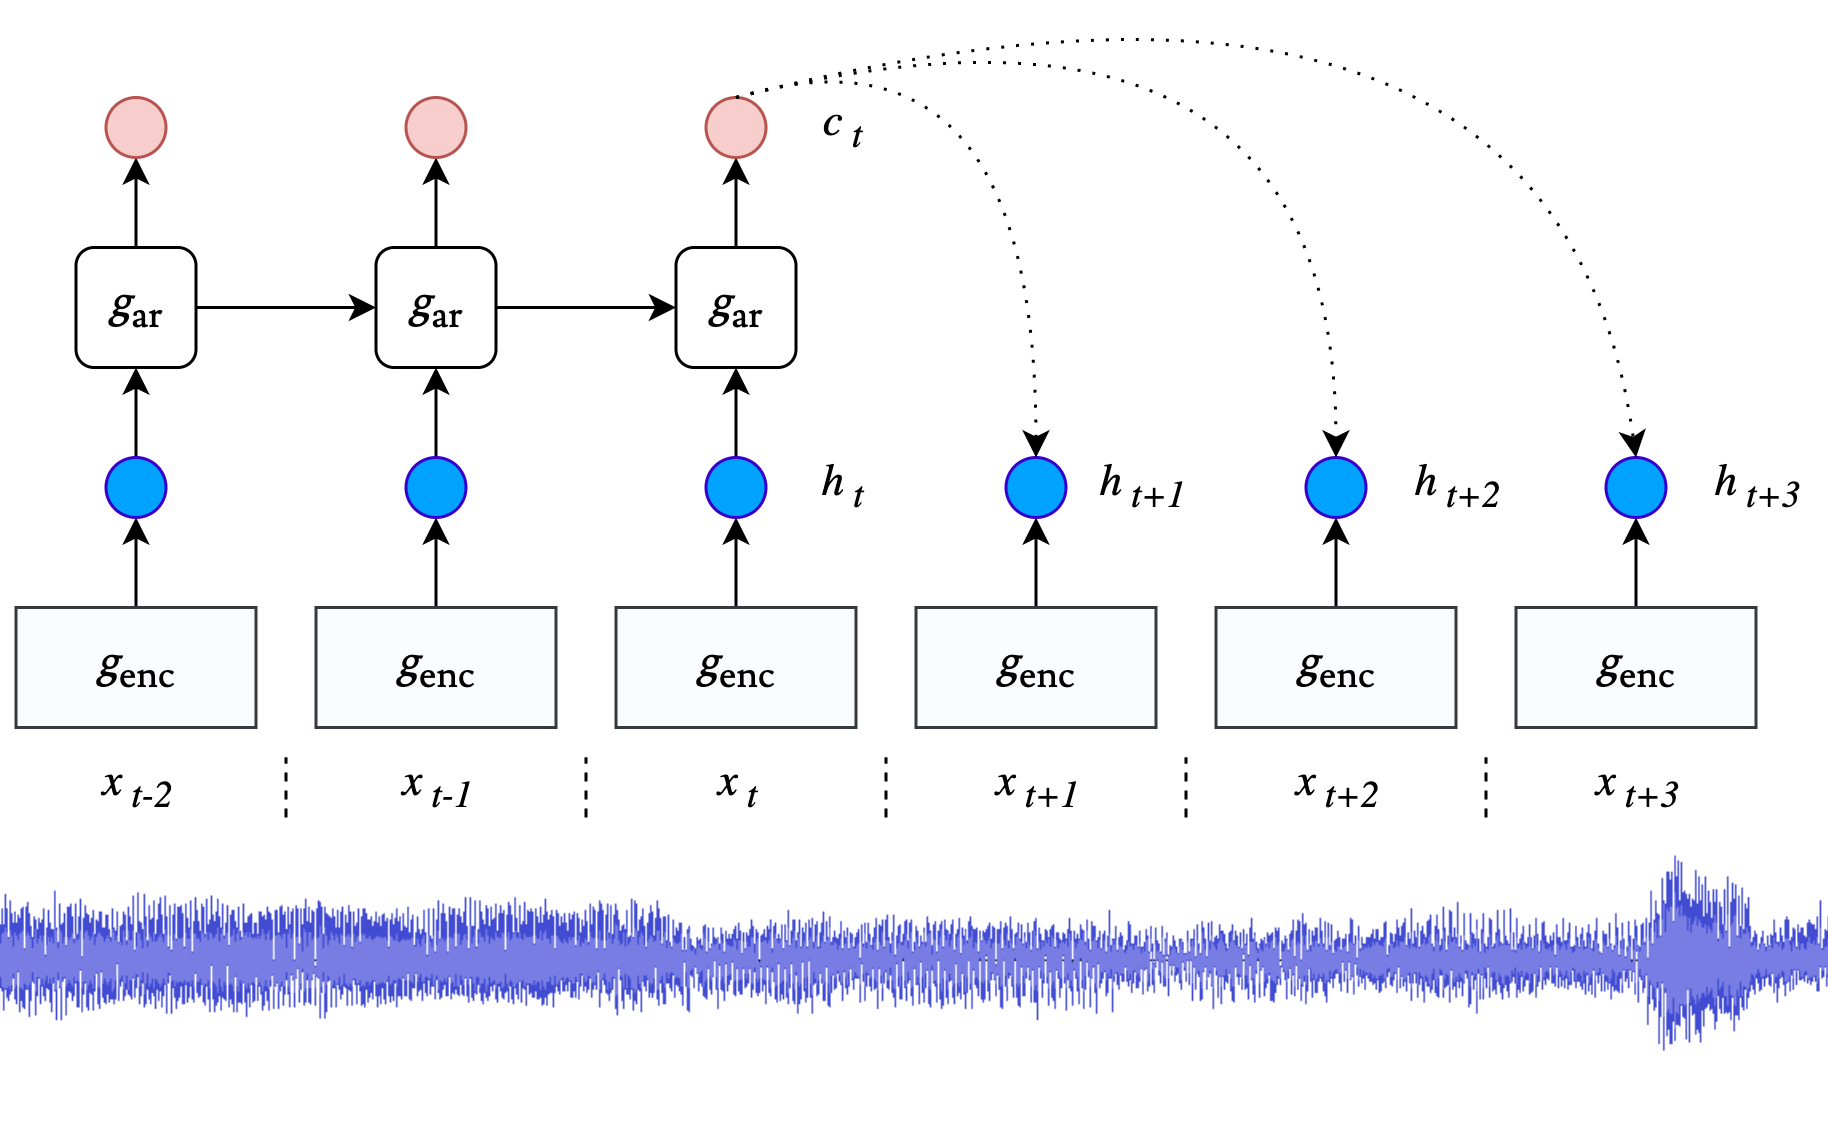
\includegraphics[width=\textwidth]{figs/cpc_model.png}
    \caption{Contrastive Predictive Coding jointly optimises two neural networks: a non-linear encoder $g_{\mathrm{enc}}$ and an autoregressor $g_{\mathrm{ar}}$, by contrasting the embeddings of temporally neighbouring patches of data using the InfoNCE loss.}
    \label{fig:cpc_model}
\end{figure}

The vectors $h_t$ and $c_t$ are encoded so as to preserve maximal mutual information and to identify the shared latent variables of the original signals. The neural networks $g_{\mathrm{enc}}(\cdot)$ and $g_{\mathrm{ar}}(\cdot)$ jointly optimise the InfoNCE loss, a contrastive loss that follows the principles of noise-contrastive estimation \cite{gutmann_noise-contrastive_nodate}. Their principles are widely used in the design of self-supervised loss functions \cite{oord_representation_2019, sohn2020fixmatch, chen_simple_2020}.

Given $N$ random samples from the set of encodings\linebreak $X = \{h_{t+k}, h_{j_1}, h_{j_2} \hdots h_N\}$, $k$ being the number of timesteps the encoding occurs after $c_t$ and $X$ containing one positive sample $h_{t+k}$ and $N-1$ negative samples $h_{j_{n}}$ drawn from representations of other samples in the same audio example and the dataset, the following objective is optimised:

\begin{equation}
    \mathcal{L}_{N}=-\sum_{k} \underset{X}{\mathbb{E}}\left[\log \frac{f_{k}\left(h_{t+k}, c_{t}\right)}{\sum_{h_{j} \in X} f_{k}\left(h_{j}, c_{t}\right)}\right]
\end{equation}

Each encoding pair $(h_n, c_t)$ is evaluated using a scoring function $f(\cdot)$ to estimate how likely a given $h_n$ is the positive sample $h_{t+k}$.
CPC's formulation of the optimal solution for $f(\cdot)$ allows $-\mathcal{L}_n$ to be reformulated as a lower bound on the mutual information of representations $I(h_{t+k} | c_t)$, which also bounds the data $I(x_{t+k} | c_t)$, and is further proven by \cite{poole_variational_2019}.
For downstream tasks, both $h_t$ and $c_t$ can be used as representations for new observations $x$, depending on whether context is helpful for solving it.

Recently, the contribution of mutual information to the success of CPC has been reconsidered: its performance depends on an inductive bias in the choice of a specialised architecture and the parameterisation of the mutual information critic \cite{Tschannen2020OnMI}.



\subsection{SimCLR}
SimCLR is a recently proposed contrastive learning technique for learning effective representations of images in a self-supervised manner without relying on specialised architectures and powerful autoregressive modeling \cite{chen_simple_2020}.
The key findings of SimCLR boils down to Yann LeCun's aforementioned `cake analogy' (\ref{fig:cake_analogy}): given a large enough neural network, a lot of unlabeled data for pre-training with a pretext task, supervised learning really becomes the icing on the cake of artificial intelligence.
Contrary to prior contrastive learning methods \cite{oord_representation_2019,henaff2019data,hjelm_learning_2019}, SimCLR does not require a specialised encoder architecture or powerful autoregressive modeling to learn useful representations. Instead, it relies on strong data augmentations and very large batch sizes to make the learned representations more rubust and the contrastive pretext task harder.
When finetuning a \textit{linear} classifier using the self-supervised learned representations from the pre-trained encoder, it achieved $76.5\%$ top-1 accuracy on ImageNet on the task of image classification.
For comparison, the same encoder architecture (ResNet-50) in a standard supervised setting scores $76.6\%$ top-1 accuracy.
A next iteration of SimCLR surpassed this supervised benchmark by a significant margin: SimCLRv2 achieves $79.8\%$ top-1 accuracy \cite{chen2020big}\footnote{BYOL surpassed the supervised benchmark a few days before SimCLRv2 was published \cite{Grill2020BootstrapYO}, but SimCLRv2 exceeded their scores.}.
\footnote{Very recently, BYOL proposed an online and target network model to mitigate the use of many negative samples \cite{Grill2020BootstrapYO}.
While they contributed interesting new findings, it goes beyond the scope of this thesis.}

The framework has four core components: 1) a composition of stochastic data augmentations that augment every image into two, correlated versions, 2) a non-linear neural network, 3) a linear or non-linear projection neural network and 4) a contrastive loss function.

The series of data augmentations the authors studied are: random cropping, resizing, horizontal flipping, cutout, color distortion (jitter, hue, dropping), gaussian noise, gaussian blur and sobel filtering. As noted earlier, the first four augmentations are considered spatial transformations, the latter four are spectral transformations.
For the sake of simplicity, they used standard ResNet encoders as the encoder neural network and feed forward neural networks for the projection layers.
Normalised temperature-scaled cross entropy loss is used as the contrastive loss function, which is shown in equation \ref{eq:loss_function}. Similarly to InfoNCE, it is a categorical cross entropy loss, but uses a different scoring function $f$ and a temperature-scaling parameter $\tau$.

\begin{equation}
    \mathcal{L} =-\log \frac{\exp \left(f\left(z_{i}, z_{j}\right) / \tau\right)}{\sum_{k=1}^{N} \mathbbm{1}_{[k \neq i]} \exp \left(f\left(z_{i}, z_{k}\right) / \tau\right)}
    \label{eq:loss_function}
\end{equation}


Batches of $2N$, i.e., every sample has a corresponding, augmented view, are used for pre-training. When training on larger batch sizes, they attribute the increased effectiveness of the learned representations to the increased complexity of the contrastive learning task. Simply put, it makes it harder for the model to infer the positive pair when increasing the pool of negative examples. With a batch size up to 8192 samples (that is 16384 samples in total during training), learning becomes unstable for standard stochastic gradient descent. To stabalise training, they employ the LARS optimiser \cite{You2017LargeBT}.

\section{CNN's for Audio}\label{sec:conv_audio}
Most papers in MIR utilise convolutional neural networks (CNN) on audio in the time-frequency domain, i.e., they use CNN's on (mel-)spectograms, CQT's, etc., to learn representations of audio \cite{chen_harmony_2019,bock_joint_2016}.
We omit describing common convolution architectures for these papers because they operate in the time-frequency domain, while our work resides in the time domain.
To learn an acoustic model from raw audio signals in the time domain, deep convolutional neural networks have proven to be useful \cite{lee2018samplecnn,pons_end--end_2017}. Large receptive fields are often used to mimic the behavior of bandpass filters, while subsequent layers control the model capacity. Auxillary layers, e.g., batch normalisation layers that suppress exploding and vanishing gradients, strong activation functions and residual connections are often deployed between convolution layers to help stabalise training for deep neural networks \cite{,he2016deep, ioffe2015batch}. Table \ref{tab:conv_block} displays a convolution block incorporating such measures.

% Musical signals are characterized well by note onsets and ensuing spectral patterns. We perform several steps of frontend processing to help learning algorithms effectively capture the features.


% \href{https://arxiv.org/pdf/1610.00087.pdf}[paper]


\begin{table}
    \centering
    \textbf{Convolution Block} \\
    \begin{tabular}{ccccc}
        \toprule Layer & Output Size \\
        & (Sequence Length $\times$ Channels) \\\hline
        Conv & h\_in $\times$ h\_out \\
        BatchNorm & h\_out \\
        ReLU & - \\
        \bottomrule
    \end{tabular}
    \caption{Convolution block consisting of a parameterised convolution layer and batch normalisation and ReLU activation layers.}
    \label{tab:conv_block}
\end{table}


\subsection{SampleCNN}
SampleCNN is a model architecture specifically designed for the classification of raw audio signals \cite{lee2018samplecnn}. It uses many layers and uses small receptive fields and aggressive pooling modules to obtain a sample-level representation of a signal \cite{lee2018samplecnn}. Its architecture is visualised in Table \ref{tab:samplecnn_model}. The kernel- and striding sizes differ slightly based on the sample rate of the input. As a trade-off between hardware constraints during training, e.g., GPU memory size, a sample rate of $22050~Hz$ yielded the highest results. This configuration's encoder, called SampleCNN $3^9$ for its pooling size and number of convolution blocks, is the default encoder used for the ablation experiments in this thesis and is shown in Figure \ref{tab:samplecnn_model}.


\begin{table*}[t]
    \centering
    \textbf{SampleCNN $3^9$ Model} \\
    \begin{tabular}{ccccc}
        \toprule Layer & Output Size & & Parameters & \\
        & (Sequence Length $\times$ Channels) & Kernel & Stride & Padding \\\hline
        Input & $59049 \times 1$ & 3 & 3 & 0 \\\hline
        ConvBlock & $19683 \times 128$ & 3 & 1 & 1 \\
        MaxPool & $6561 \times 128$ & 3 & 3 & 1 \\\hline
        ConvBlock & $6561 \times 128$ & 3 & 1 & 1 \\
        MaxPool & $2187 \times 256$ & 3 & 3 & 1 \\\hline
        ConvBlock & $2187 \times 256$ & 3 & 1 & 1 \\
        MaxPool & $729 \times 256$ & 3 & 3 & 1 \\\hline
        ConvBlock & $729 \times 256$ & 3 & 1 & 1 \\
        MaxPool & $243 \times 256$ & 3 & 3 & 1 \\\hline
        ConvBlock & $243 \times 256$ & 3 & 1 & 1 \\
        MaxPool & $81 \times 256$ & 3 & 3 & 1 \\\hline
        ConvBlock & $81 \times 256$ & 3 & 1 & 1 \\
        MaxPool & $27 \times 256$ & 3 & 3 & 1 \\\hline
        ConvBlock & $27 \times 256$ & 3 & 1 & 1 \\
        MaxPool & $9 \times 256$ & 3 & 3 & 1 \\\hline
        ConvBlock & $9 \times 512$ & 3 & 1 & 1 \\
        MaxPool & $3 \times 512$ & 3 & 3 & 1 \\\hline
        ConvBlock & $3 \times 512$ & 3 & 1 & 1 \\
        MaxPool & $1 \times 512$ & 3 & 3 & 1 \\\hline
        ConvBlock & $1 \times 512$ & 3 & 1 & 1 \\
        Dropout (0.5) & $1 \times 512$ & - & - & - \\\hline
        FC & 50 & - & - & - \\
        \bottomrule
    \end{tabular}
    \caption[][15pt]{SampleCNN $3^9$ Model, with 59049 samples (2678~ms) as input.
Each ConvBlock consists of the modules presented in Table \ref{tab:conv_block}}
    \label{tab:samplecnn_model}
\end{table*}


\section{Music Tagging}\label{sec:task_description}
Music (auto) tagging, or music classification, is the task of automatically attributing metadata to a fragment of musical audio.
The attribution can be a single genre or multiple `tags' that best describe the contents of the signal.
The type of task can thus either be a multi-class or multi-label classification problem.
The attributes range from tags that describe the (1) genre, e.g., jazz, pop, metal, (2) moods, e.g., happy, sad, (3) instruments, e.g., guitar, piano, harp, or (4) even more semantic descriptions, e.g., beautiful, of a fragment of music.

The idea behind choosing this downstream task, is that the contrastive learning objective lends itself to such a discriminative task.
Moreover, music tags describe many facets of music. When a self-supervised model is able to learn an effective mapping of the versatility of such semantic tasks on high-dimensional signals, it paves the way for more specific musical tasks, e.g., chord recognition. 
\footnote{The initial idea in this thesis was to evaluate more downstream musical tasks under the learned representations by a self-supervised model, but we quickly found that focussing on one task in such an unexplored field was enough, and leave the evaluation of other tasks for future research.}


% These attributes may include: moods, language of the lyrics, year of composition, genre(s), instruments, harmony traits, or rhythmic traits.

% Front-ends. These are generally conformed by convolutional neural networks (CNNs) [4, 2, 13, 8, 9],
% since these can learn efficient representations by sharing weights (feature representations) along the
% signal. Generally, a single filter shape is used in the first CNN layer [4, 2, 5], but some recent work
% reported performance gains when using several filter shapes in the first layer [13, 8, 9]. Using many
% filters facilitates leveraging domain knowledge for designing the filters’ shape, and also promotes a
% more rich feature extraction in the first layer – where the signal is available. Further, the design of the
% filters can be either based on domain knowledge or not. For example, one leverages domain knowledge
% when a waveform front-end is designed so that the length of the filter is set to be the same as the
% window length in a STFT [4].

\subsection{Evaluation Metrics}
To directly compare the results of this thesis with prior work \cite{dieleman2014end,lee2018samplecnn,pons_end--end_2017}, we employ the $\mathrm{ROC-AUC}_{\mathrm{TAG}}$ and $\mathrm{PR-AUC}_{\mathrm{TAG}}$ evaluation metrics. The ROC-AUC is the area under the receiver operating characteristic curve that evaluates binary classification problems by summarising the True Positive and False Positive rates. An ROC-AUC score of 1 means the classifier is able to perfectly distinguish true- from false positive labels. When 0, the classifier predicts exactly every true positive as a false positive class and the other way around. With an ROC-AUC of 0.5, the classifier is unable to distinguish between true- and false positive classes. The ROC-AUC metric suffers over-optimistic scores when classes are inbalanced in the dataset \cite{rocaucimbalance}. We therefore also employ the PR-AUC evaluation metric, which measures the area under the precision-recall curve. The precision indicates how many correct positive predictions are made. Recall quantifies the number of relevant correct predictions.

As the subscripts in both metrics show, we measure the TAG performance on our task, but also measure the CLIP performance. The evaluation metrics are measured globally for the whole dataset, i.e., for the tag metric we measure the retrieval performance on the tag dimension (column-wise) and for the clip metric we measure the performance on the clip dimension (row-wise). Intuitively, the tag retrieval performance tells us how well the model is able to correctly retrieve all the music fragments (clips), given the tags, while the clip retrieval performance how well the model retrieves all tags given a clip.

\section*{Summary}
In this chapter, we recapitulated the foundations which are used to build on in this thesis. We gave a brief overview of the different strategies of representation learning to clarify self-supervised learning, i.e., a form of unsupervised learning that formulates the learning objective so that it retrieves a supervisory signal from (transformations of) the data itself. We gave a more extensive description of existing literature on self-supervised learning, important pretext tasks and their strengths, and made an important distinction between learning spectral and spatial relationships when only using a pretext task to learn on data. Subsequently, we addressed self-supervised learning techniques in the audio domain and detailed some of the audio transformation pipelines and augmentations used in the literature. We discussed the contrastive learning paradigm within self-supervised learning, detailing contrastive predictive coding, SimCLR, and noise-contrastive estimation losses. We discussed encoders used in the literature on deep learning on audio in the time domain, and described the SampleCNN model which is used in this thesis. Finally, we gave a description of the evalation metrics we used to evaluate the performance of our proposed self-supervised model on raw audio: CLMR.